%!TEX root = ../thesis.tex

\section{実験1}
\subsection{実験目的}
シミュレータ上で実験を行い, 提案手法の有効性を検証する.

\subsection{実験装置}
aaa実験は, \figref{Fig:gazebo}に示すGazebo\cite{gazebo}のWillow Garage\cite{willow}で\figref{Fig:willow-garage}に示すコースで一周行う. また, ロボットモデルには\figref{Fig:turtlebot3}に示すようなカメラを3つ搭載したTurtlebot3\cite{turtlebot3}を用いた. 

\begin{figure}[h]
  \centering
  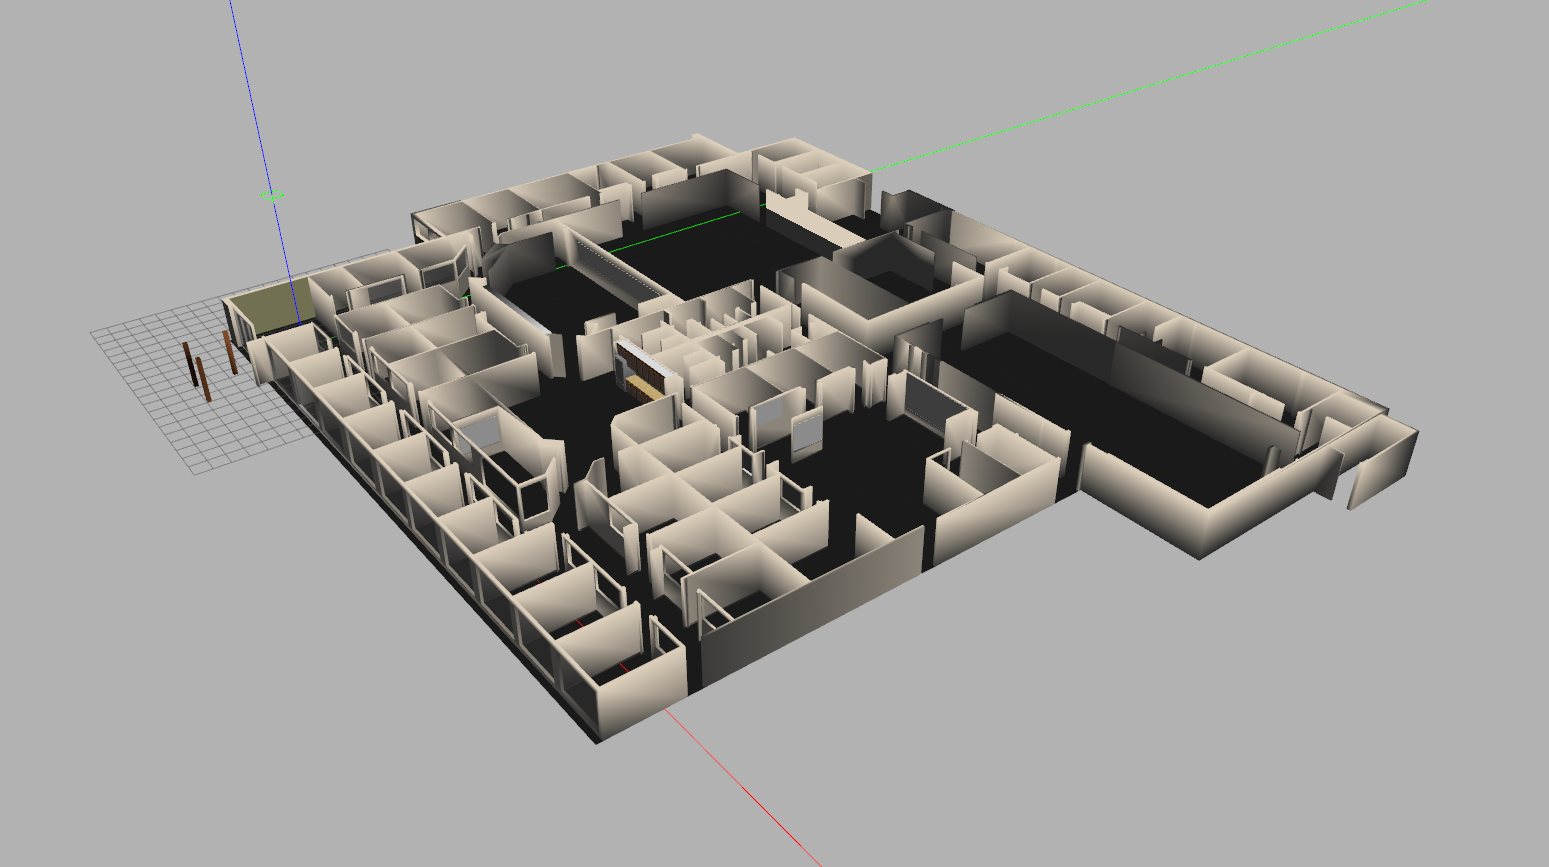
\includegraphics[keepaspectratio, scale=0.15]{images/gazebo.png}
  \caption{Experimental environment in simulator}
  \label{Fig:gazebo}
  \end{figure}

\newpage
\vspace{20mm}
\begin{figure}[h]
  \centering
  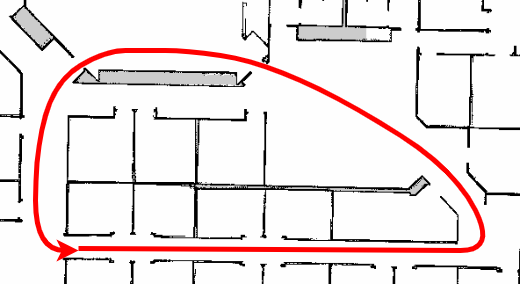
\includegraphics[keepaspectratio, scale=0.5]{images/willow-path.png}
  \caption{Course to collect data}
  \label{Fig:willow-garage}
  \end{figure}

\begin{figure}[h]
  \centering
  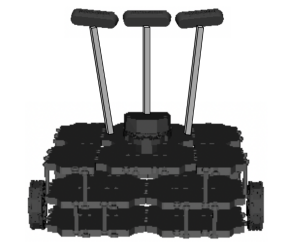
\includegraphics[keepaspectratio, scale=0.55]{images/turtlebot3.png}
  \caption{Turtlebot3 waffle with 3 cameras}
  \label{Fig:turtlebot3}
  \end{figure}

\newpage
\subsection{実験方法}
\begin{description}
  \item[1.データ収集フェーズ]\mbox{}\\データの収集方法について述べる. \figref{Fig:old-method}にデータの収集方法を示す. 赤色の線である目標経路から平行に±0.10, ±0.20, ±0.30m, また, ロボットの進行方向に対しては0.5m離れた座標にロボットを配置する. そして, その座標ごとに目標経路に沿った向きを基準として±5度傾けて, カメラ画像とナビゲーションの出力である角速度を収集する. これを\figref{Fig:willow-garage}に示した経路で実験を行う. 
\end{description}

\begin{figure}[h]
  \centering
  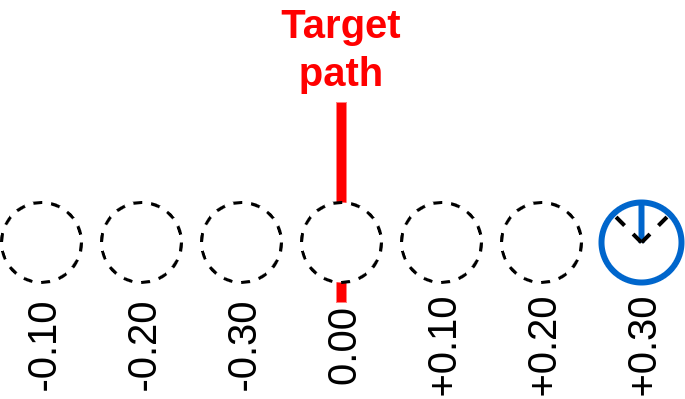
\includegraphics[keepaspectratio, scale=0.25]{images/old-method.png}
  \caption{Method of collecting data around the target route}
  \label{Fig:old-method}
  \end{figure}

\begin{description}
  \item[2.訓練フェーズ]\mbox{}\\データ収集フェーズで収集したデータ2748個を用いて, バッチ学習で4000step, 8000step, 10000step学習した. なお, 4000stepは従来手法において, シミュレータの実験に用いられてきたステップ数であり, 10000stepは従来手法において, 実ロボットの実験に用いられていたステップ数である. 
\end{description}

\begin{description}
  \item[3.テストフェーズ]\mbox{}\\ \figref{Fig:willow-garage}に示すコースで10個の学習済みモデルを使用して走行させる. ロボットの並進速度0.2m/sとし, 経路を3周できた場合を成功, 壁に激突したり, 経路から10m離れたりした場合を失敗とした.
\end{description}

\subsection{実験結果}
実験結果を表\ref{tb:exp1.2}に示す. また, 失敗箇所は\figref{Fig:result1.2}, 失敗箇所ごとの失敗回数は表\ref{tb:fail1.2}のようになった. 
\par \figref{Fig:result1.2}の×の箇所で曲がり切ることができずにコースアウトしてしまった. 訓練時のlossを\figref{Fig:exp1.2_4000}, \figref{Fig:exp1.2_8000}, \figref{Fig:exp1.2_10000}に示す. 図では. 学習が収束している様子が確認できる. ここで, 角を曲がりきれなかった要因の一つとして, コースアウトした箇所付近の目標経路周辺のデータが足りないためだと考えられる. また, ステップ数を増やして成功回数が減ったのは, 直進のデータを多く学習しすぎて過学習を起こしている可能性もある. これを踏まえて, 次に目標経路と平行な方向のロボットの配置間隔を狭めて, データ数を増やすことで成功回数が増えるか検証する. 

\begin{table}[h]
  \centering
  \caption{Number of successes in the batch learning}
  \begin{tabular}{|c|c|} \hline
    Experiments & Number of successes \\ \hline
    Exp.1(4000step) & 4/10 \\ \hline
    Exp.2(8000step) & 2/10 \\ \hline
    Exp.3(10000step) & 2/10 \\ \hline
  \end{tabular}
  \label{tb:exp1.2}
\end{table}

\begin{figure}[h]
  \centering
  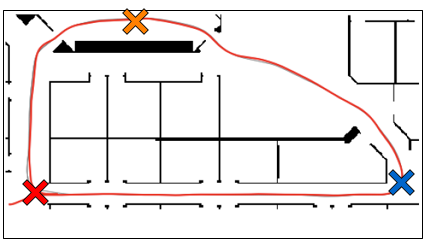
\includegraphics[keepaspectratio, scale=0.5]{images/result1.2.png}
  \caption{Failure point of the experiment}
  \label{Fig:result1.2}
  \end{figure}

\newpage
\begin{table}[h]
  \centering
  \caption{Number of failures in the experiment}
  \begin{tabular}{|c|c|c|c|} \hline
    Experiments & Failures with blue x & Failures with red x & Failures with orange x\\ \hline
    Exp.1(4000step) & 1 & 5 & 0 \\ \hline
    Exp.2(8000step) & 1 & 7 & 0 \\ \hline
    Exp.3(10000step) & 1 & 5 & 2 \\ \hline
  \end{tabular}
  \label{tb:fail1.2}
\end{table}

\vspace{20mm}
\begin{figure}[h]
  \centering
  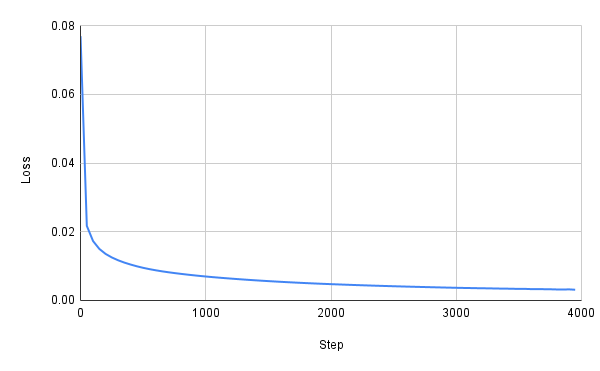
\includegraphics[keepaspectratio, scale=0.5]{images/exp1.2_4000.png}
  \caption{Loss value in the experiment1}
  \label{Fig:exp1.2_4000}
  \end{figure}
  
\begin{figure}[h]
  \centering
  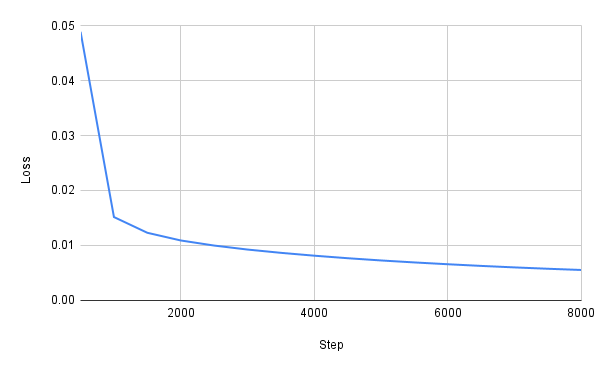
\includegraphics[keepaspectratio, scale=0.5]{images/exp1.2_8000.png}
  \caption{Loss value in the experiment2}
  \label{Fig:exp1.2_8000}
  \end{figure}

  \newpage
\begin{figure}[h]
  \centering
  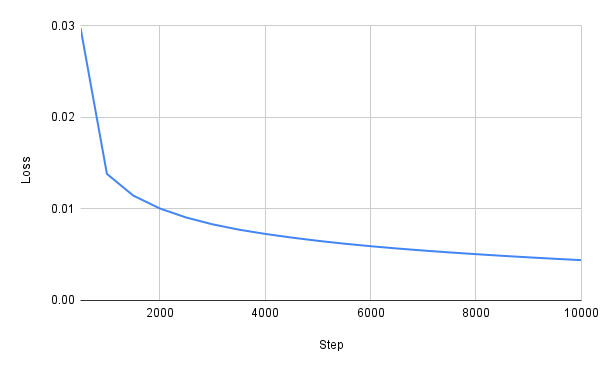
\includegraphics[keepaspectratio, scale=0.5]{images/exp1.2_10000.png}
  \caption{Loss value in the experiment3}
  \label{Fig:exp1.2_10000}
  \end{figure}

\newpage
\section{実験2}
実験目的, 実験装置, テストフェーズは実験1と同様である.
\subsection{実験方法}
\begin{description}
  \item[1.データ収集フェーズ]\mbox{}\\実験1を踏まえて, 経路周辺のデータを多く取得する手法を試みる. \figref{Fig:collect-data}にデータの収集方法を示す. 赤色の線である目標経路から平行に±0.01, ±0.02, ±0.04, ±0.06, ±0.08, ±0.10, ±0.15, ±0.20, ±0.30m離れた座標にロボットを配置する. そして, 手法1と同様にロボットを傾けて画像と角速度を\figref{Fig:collect-data2}のように収集する. これを\figref{Fig:willow-garage}に示すコースで一周行う.  
\end{description}

\begin{figure}[h]
  \centering
  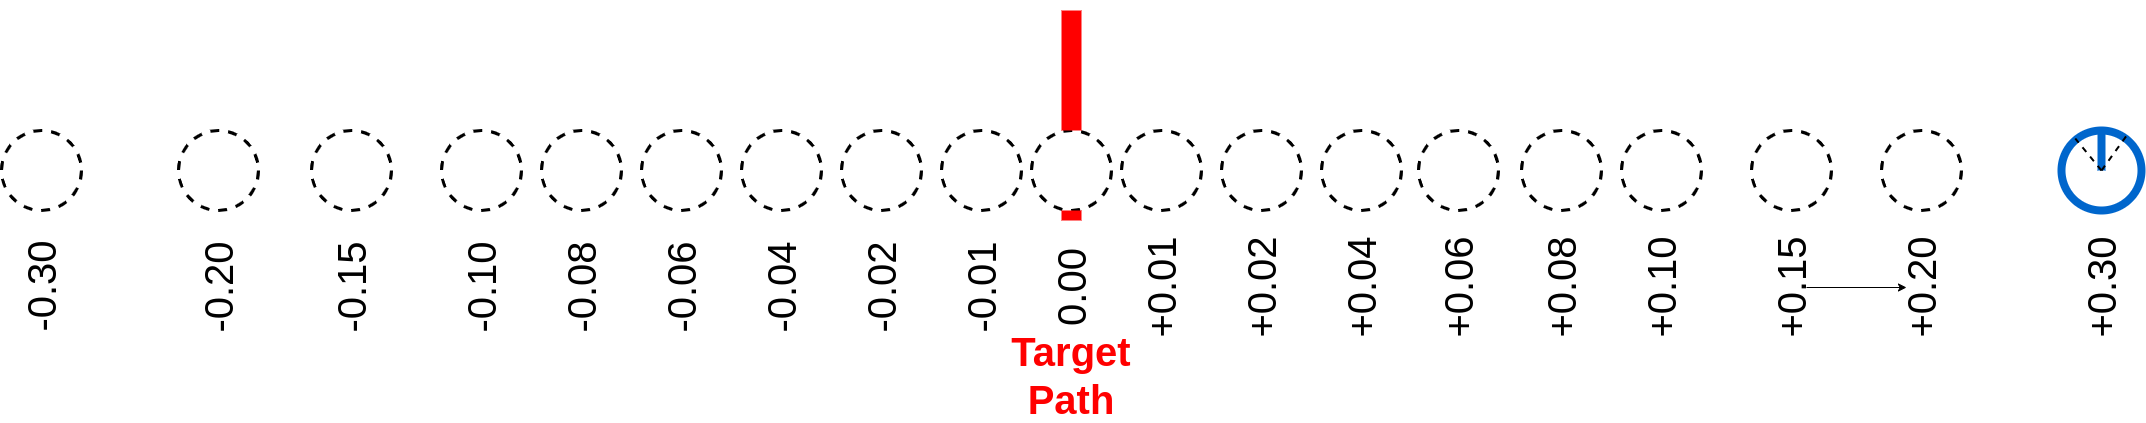
\includegraphics[keepaspectratio, scale=0.18]{images/collect-data.png}
  \caption{Method of collecting data around the target route}
  \label{Fig:collect-data}
  \end{figure}

\begin{description}
  \item[2.訓練フェーズ]\mbox{}\\データ収集フェーズで収集したデータ7452個を用いて, バッチ学習で4000step, 8000step, 10000step学習した. 
\end{description}

\newpage
\subsection{実験結果}
実験結果を表\ref{tb:exp2.2}に示す. 実験1と実験2で収集した角速度のデータ数の比率を\figref{Fig:hist}に示す. 実験2では, 収集したデータ数全体の数も増えているが, 角を曲がる際の角速度0.3rad/s以上のデータも増えていることが分かる. また, 4000step, 8000step, 10000step全てで成功回数が10/10となり, 経路を周回することができた. ここで, 学習のlossを\figref{Fig:exp2.2-4000}, \figref{Fig:exp2.2-8000}, \figref{Fig:exp2.2-10000}に示す.\figref{Fig:exp2.2-4000}, \figref{Fig:exp2.2-8000}, \figref{Fig:exp2.2-10000}はステップ数を増やすに連れて, 学習が収束している様子を確認できる. 従って, 目標経路周辺においてロボットの配置間隔を狭め, バッチ学習を用いて訓練することで経路追従できることを確認した. 

\vspace{10mm}
\begin{table}[h]
  \centering
  \caption{Number of successes in the experiment}
  \begin{tabular}{|c|c|} \hline
    Experiments & Number of successes \\ \hline
    Exp.1(4000step) & 10/10 \\ \hline
    Exp.2(8000step) & 10/10 \\ \hline
    Exp.3(10000step) & 10/10 \\ \hline
  \end{tabular}
  \label{tb:exp2.2}
\end{table}

\newpage
\begin{figure}[h]
  \centering
  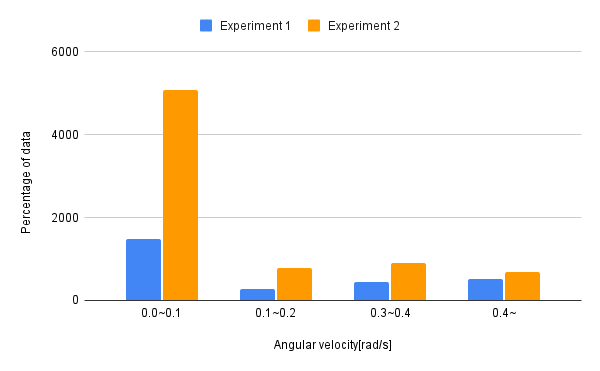
\includegraphics[keepaspectratio, scale=0.53]{images/ang_sum.png}
  \caption{Histogram of collected angular velocities in the experiment1 and the experiment2}
  \label{Fig:hist}
  \end{figure}

\begin{figure}[h]
  \centering
  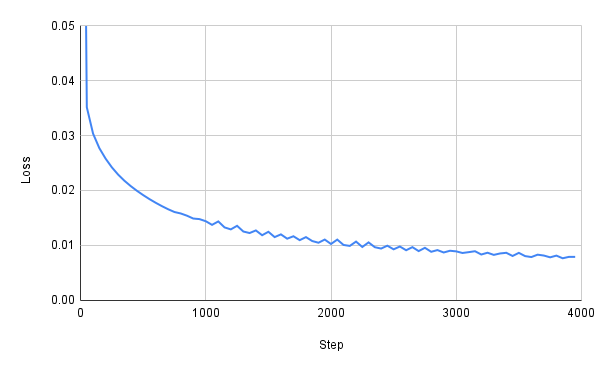
\includegraphics[keepaspectratio, scale=0.5]{images/exp3_4000_fix.png}
  \caption{Loss value in the experiment1}
  \label{Fig:exp2.2-4000}
  \end{figure}

\begin{figure}[h]
  \centering
  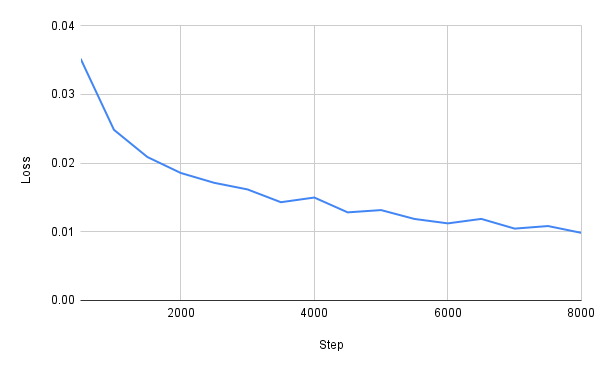
\includegraphics[keepaspectratio, scale=0.5]{images/exp3_8000.png}
  \caption{Loss value in the experiment2}
  \label{Fig:exp2.2-8000}
  \end{figure}

\newpage
\begin{figure}[h]
  \centering
  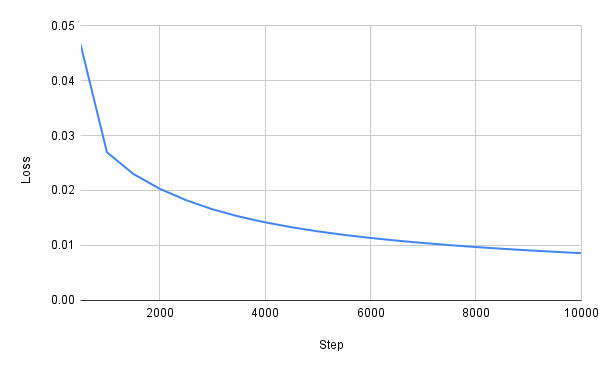
\includegraphics[keepaspectratio, scale=0.5]{images/exp3_10000.png}
  \caption{Loss value in the experiment3}
  \label{Fig:exp2.2-10000}
  \end{figure}

\newpage
\section{実験3}
ここでは, 実験2で成功率が100\%であった4000stepから1000stepずつステップ数を減らした場合に, 成功率及び訓練時間がどのように変わるか検証する. 実験目的, 実験装置, データ収集フェーズ, テストフェーズは実験2と同様である. 

\subsection{実験方法}
\begin{description}
  \item[2.訓練フェーズ]\mbox{}\\データ数7452, バッチ学習で4000step, 3000step, 2000step, 1000step学習した. 
\end{description}

\subsection{実験結果}
実験結果を表\ref{tb:exp3}を示す. 失敗箇所は\figref{Fig:result3}, 失敗箇所ごとの失敗回数を表\ref{tb:fail3}に示す. 3000stepでは成功率90\%, 4分40秒で訓練が終了した. 2000stepでは成功率80\%, 3分10秒で訓練が終了し, 4000stepの半分の時間で訓練を終了することができた. また, 1000stepでは成功率は50\%であったが, 4000step訓練するのに必要としていた時間を約25\%で削減することができた. ここで, 各ステップ数ごとのlossを\figref{Fig:3000}, \figref{Fig:2000}, \figref{Fig:1000}に示す. 結果として, 従来手法が訓練に最低約40分程度必要であったのに対して, 大幅に時間を短縮できることを確認した. 

\vspace{10mm}
\begin{table}[h]
  \centering
  \caption{Number of successes in the experiment}
  \begin{tabular}{|c|c|c|} \hline
    Experiments & Number of successes & Time required for learning\\ \hline
    Exp.1(4000step) & 10/10 & 6min. 20sec.\\ \hline
    Exp.2(3000step) & 9/10 & 4min. 40sec.\\ \hline
    Exp.3(2000step) & 8/10 & 3min. 10sec.\\ \hline
    Exp.4(1000step) & 5/10 & 1min. 34sec.\\ \hline
  \end{tabular}
  \label{tb:exp3}
\end{table}

\begin{figure}[h]
  \centering
  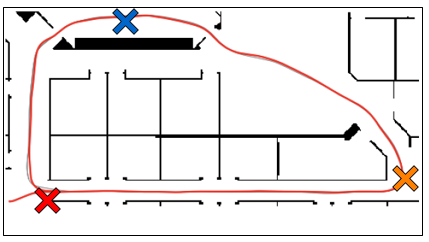
\includegraphics[keepaspectratio, scale=0.5]{images/result4.png}
  \caption{Failure point of the experiment}
  \label{Fig:result3}
  \end{figure}

\begin{table}[h]
  \centering
  \caption{Number of failures in the experiment}
  \begin{tabular}{|c|c|c|c|} \hline
    Experiments & Failures with blue x & Failures with red x & Failures with orange x\\ \hline
    Exp.2(3000step) & 1 & 0 & 0 \\ \hline
    Exp.3(2000step) & 1 & 1 & 0 \\ \hline
    Exp.4(1000step) & 4 & 0 & 1 \\ \hline
  \end{tabular}
  \label{tb:fail3}
\end{table}

\begin{figure}[h]
  \centering
  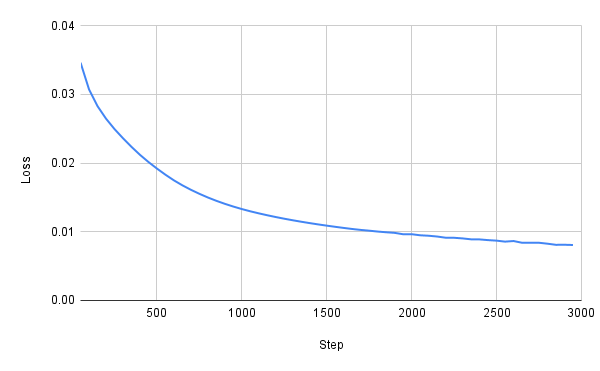
\includegraphics[keepaspectratio, scale=0.5]{images/3000.png}
  \caption{Loss value in the experiments}
  \label{Fig:3000}
  \end{figure}

\begin{figure}[h]
  \centering
  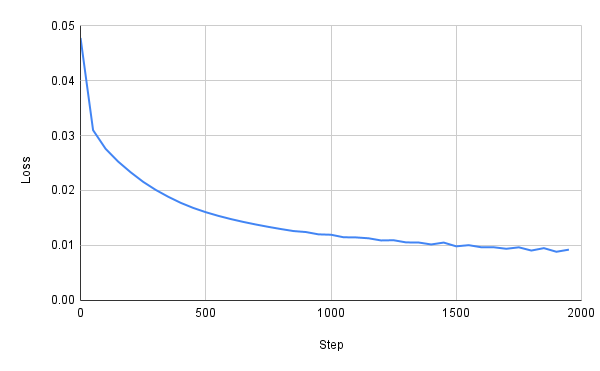
\includegraphics[keepaspectratio, scale=0.5]{images/2000.png}
  \caption{Loss value in the experiments}
  \label{Fig:2000}
  \end{figure}

\begin{figure}[h]
  \centering
  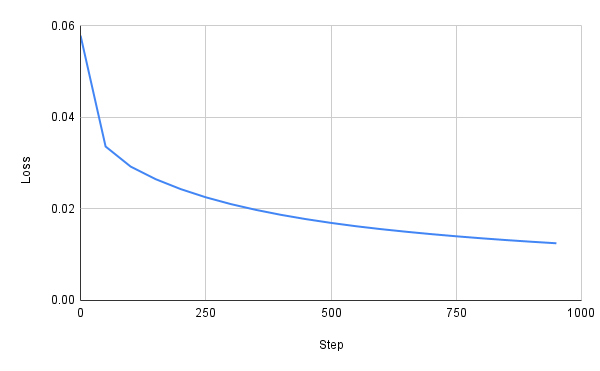
\includegraphics[keepaspectratio, scale=0.5]{images/1000.png}
  \caption{Loss value in the experiments}
  \label{Fig:1000}
  \end{figure}